% Graphic for TeX using PGF
% Title: /home/aleix/upc/pfc_svn/imatges/model/roundrobinson-uml.dia
% Creator: Dia v0.97.1
% CreationDate: Sun Jul  3 19:04:13 2011
% For: aleix
% \usepackage{tikz}
% The following commands are not supported in PSTricks at present
% We define them conditionally, so when they are implemented,
% this pgf file will use them.
\ifx\du\undefined
  \newlength{\du}
\fi
\setlength{\du}{15\unitlength}
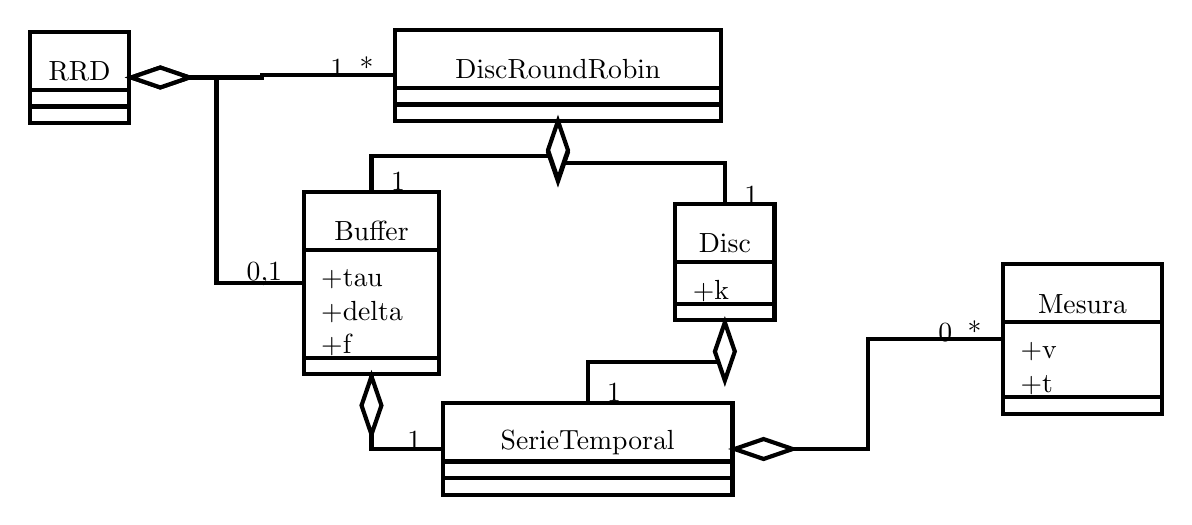
\begin{tikzpicture}
\pgftransformxscale{1.000000}
\pgftransformyscale{-1.000000}
\definecolor{dialinecolor}{rgb}{0.000000, 0.000000, 0.000000}
\pgfsetstrokecolor{dialinecolor}
\definecolor{dialinecolor}{rgb}{1.000000, 1.000000, 1.000000}
\pgfsetfillcolor{dialinecolor}
\pgfsetlinewidth{0.100000\du}
\pgfsetdash{}{0pt}
\definecolor{dialinecolor}{rgb}{1.000000, 1.000000, 1.000000}
\pgfsetfillcolor{dialinecolor}
\fill (21.850000\du,0.700000\du)--(21.850000\du,2.100000\du)--(25.667500\du,2.100000\du)--(25.667500\du,0.700000\du)--cycle;
\definecolor{dialinecolor}{rgb}{0.000000, 0.000000, 0.000000}
\pgfsetstrokecolor{dialinecolor}
\draw (21.850000\du,0.700000\du)--(21.850000\du,2.100000\du)--(25.667500\du,2.100000\du)--(25.667500\du,0.700000\du)--cycle;
% setfont left to latex
\definecolor{dialinecolor}{rgb}{0.000000, 0.000000, 0.000000}
\pgfsetstrokecolor{dialinecolor}
\node at (23.758750\du,1.650000\du){Mesura};
\definecolor{dialinecolor}{rgb}{1.000000, 1.000000, 1.000000}
\pgfsetfillcolor{dialinecolor}
\fill (21.850000\du,2.100000\du)--(21.850000\du,3.900000\du)--(25.667500\du,3.900000\du)--(25.667500\du,2.100000\du)--cycle;
\definecolor{dialinecolor}{rgb}{0.000000, 0.000000, 0.000000}
\pgfsetstrokecolor{dialinecolor}
\draw (21.850000\du,2.100000\du)--(21.850000\du,3.900000\du)--(25.667500\du,3.900000\du)--(25.667500\du,2.100000\du)--cycle;
% setfont left to latex
\definecolor{dialinecolor}{rgb}{0.000000, 0.000000, 0.000000}
\pgfsetstrokecolor{dialinecolor}
\node[anchor=west] at (22.000000\du,2.800000\du){+v};
% setfont left to latex
\definecolor{dialinecolor}{rgb}{0.000000, 0.000000, 0.000000}
\pgfsetstrokecolor{dialinecolor}
\node[anchor=west] at (22.000000\du,3.600000\du){+t};
\definecolor{dialinecolor}{rgb}{1.000000, 1.000000, 1.000000}
\pgfsetfillcolor{dialinecolor}
\fill (21.850000\du,3.900000\du)--(21.850000\du,4.300000\du)--(25.667500\du,4.300000\du)--(25.667500\du,3.900000\du)--cycle;
\definecolor{dialinecolor}{rgb}{0.000000, 0.000000, 0.000000}
\pgfsetstrokecolor{dialinecolor}
\draw (21.850000\du,3.900000\du)--(21.850000\du,4.300000\du)--(25.667500\du,4.300000\du)--(25.667500\du,3.900000\du)--cycle;
\pgfsetlinewidth{0.100000\du}
\pgfsetdash{}{0pt}
\definecolor{dialinecolor}{rgb}{1.000000, 1.000000, 1.000000}
\pgfsetfillcolor{dialinecolor}
\fill (8.350000\du,4.050000\du)--(8.350000\du,5.450000\du)--(15.327500\du,5.450000\du)--(15.327500\du,4.050000\du)--cycle;
\definecolor{dialinecolor}{rgb}{0.000000, 0.000000, 0.000000}
\pgfsetstrokecolor{dialinecolor}
\draw (8.350000\du,4.050000\du)--(8.350000\du,5.450000\du)--(15.327500\du,5.450000\du)--(15.327500\du,4.050000\du)--cycle;
% setfont left to latex
\definecolor{dialinecolor}{rgb}{0.000000, 0.000000, 0.000000}
\pgfsetstrokecolor{dialinecolor}
\node at (11.838750\du,5.000000\du){SerieTemporal};
\definecolor{dialinecolor}{rgb}{1.000000, 1.000000, 1.000000}
\pgfsetfillcolor{dialinecolor}
\fill (8.350000\du,5.450000\du)--(8.350000\du,5.850000\du)--(15.327500\du,5.850000\du)--(15.327500\du,5.450000\du)--cycle;
\definecolor{dialinecolor}{rgb}{0.000000, 0.000000, 0.000000}
\pgfsetstrokecolor{dialinecolor}
\draw (8.350000\du,5.450000\du)--(8.350000\du,5.850000\du)--(15.327500\du,5.850000\du)--(15.327500\du,5.450000\du)--cycle;
\definecolor{dialinecolor}{rgb}{1.000000, 1.000000, 1.000000}
\pgfsetfillcolor{dialinecolor}
\fill (8.350000\du,5.850000\du)--(8.350000\du,6.250000\du)--(15.327500\du,6.250000\du)--(15.327500\du,5.850000\du)--cycle;
\definecolor{dialinecolor}{rgb}{0.000000, 0.000000, 0.000000}
\pgfsetstrokecolor{dialinecolor}
\draw (8.350000\du,5.850000\du)--(8.350000\du,6.250000\du)--(15.327500\du,6.250000\du)--(15.327500\du,5.850000\du)--cycle;
\pgfsetlinewidth{0.100000\du}
\pgfsetdash{}{0pt}
\definecolor{dialinecolor}{rgb}{1.000000, 1.000000, 1.000000}
\pgfsetfillcolor{dialinecolor}
\fill (5.000000\du,-1.050000\du)--(5.000000\du,0.350000\du)--(8.265000\du,0.350000\du)--(8.265000\du,-1.050000\du)--cycle;
\definecolor{dialinecolor}{rgb}{0.000000, 0.000000, 0.000000}
\pgfsetstrokecolor{dialinecolor}
\draw (5.000000\du,-1.050000\du)--(5.000000\du,0.350000\du)--(8.265000\du,0.350000\du)--(8.265000\du,-1.050000\du)--cycle;
% setfont left to latex
\definecolor{dialinecolor}{rgb}{0.000000, 0.000000, 0.000000}
\pgfsetstrokecolor{dialinecolor}
\node at (6.632500\du,-0.100000\du){Buffer};
\definecolor{dialinecolor}{rgb}{1.000000, 1.000000, 1.000000}
\pgfsetfillcolor{dialinecolor}
\fill (5.000000\du,0.350000\du)--(5.000000\du,2.950000\du)--(8.265000\du,2.950000\du)--(8.265000\du,0.350000\du)--cycle;
\definecolor{dialinecolor}{rgb}{0.000000, 0.000000, 0.000000}
\pgfsetstrokecolor{dialinecolor}
\draw (5.000000\du,0.350000\du)--(5.000000\du,2.950000\du)--(8.265000\du,2.950000\du)--(8.265000\du,0.350000\du)--cycle;
% setfont left to latex
\definecolor{dialinecolor}{rgb}{0.000000, 0.000000, 0.000000}
\pgfsetstrokecolor{dialinecolor}
\node[anchor=west] at (5.150000\du,1.050000\du){+tau};
% setfont left to latex
\definecolor{dialinecolor}{rgb}{0.000000, 0.000000, 0.000000}
\pgfsetstrokecolor{dialinecolor}
\node[anchor=west] at (5.150000\du,1.850000\du){+delta};
% setfont left to latex
\definecolor{dialinecolor}{rgb}{0.000000, 0.000000, 0.000000}
\pgfsetstrokecolor{dialinecolor}
\node[anchor=west] at (5.150000\du,2.650000\du){+f};
\definecolor{dialinecolor}{rgb}{1.000000, 1.000000, 1.000000}
\pgfsetfillcolor{dialinecolor}
\fill (5.000000\du,2.950000\du)--(5.000000\du,3.350000\du)--(8.265000\du,3.350000\du)--(8.265000\du,2.950000\du)--cycle;
\definecolor{dialinecolor}{rgb}{0.000000, 0.000000, 0.000000}
\pgfsetstrokecolor{dialinecolor}
\draw (5.000000\du,2.950000\du)--(5.000000\du,3.350000\du)--(8.265000\du,3.350000\du)--(8.265000\du,2.950000\du)--cycle;
\pgfsetlinewidth{0.100000\du}
\pgfsetdash{}{0pt}
\definecolor{dialinecolor}{rgb}{1.000000, 1.000000, 1.000000}
\pgfsetfillcolor{dialinecolor}
\fill (13.950000\du,-0.750000\du)--(13.950000\du,0.650000\du)--(16.340000\du,0.650000\du)--(16.340000\du,-0.750000\du)--cycle;
\definecolor{dialinecolor}{rgb}{0.000000, 0.000000, 0.000000}
\pgfsetstrokecolor{dialinecolor}
\draw (13.950000\du,-0.750000\du)--(13.950000\du,0.650000\du)--(16.340000\du,0.650000\du)--(16.340000\du,-0.750000\du)--cycle;
% setfont left to latex
\definecolor{dialinecolor}{rgb}{0.000000, 0.000000, 0.000000}
\pgfsetstrokecolor{dialinecolor}
\node at (15.145000\du,0.200000\du){Disc};
\definecolor{dialinecolor}{rgb}{1.000000, 1.000000, 1.000000}
\pgfsetfillcolor{dialinecolor}
\fill (13.950000\du,0.650000\du)--(13.950000\du,1.650000\du)--(16.340000\du,1.650000\du)--(16.340000\du,0.650000\du)--cycle;
\definecolor{dialinecolor}{rgb}{0.000000, 0.000000, 0.000000}
\pgfsetstrokecolor{dialinecolor}
\draw (13.950000\du,0.650000\du)--(13.950000\du,1.650000\du)--(16.340000\du,1.650000\du)--(16.340000\du,0.650000\du)--cycle;
% setfont left to latex
\definecolor{dialinecolor}{rgb}{0.000000, 0.000000, 0.000000}
\pgfsetstrokecolor{dialinecolor}
\node[anchor=west] at (14.100000\du,1.350000\du){+k};
\definecolor{dialinecolor}{rgb}{1.000000, 1.000000, 1.000000}
\pgfsetfillcolor{dialinecolor}
\fill (13.950000\du,1.650000\du)--(13.950000\du,2.050000\du)--(16.340000\du,2.050000\du)--(16.340000\du,1.650000\du)--cycle;
\definecolor{dialinecolor}{rgb}{0.000000, 0.000000, 0.000000}
\pgfsetstrokecolor{dialinecolor}
\draw (13.950000\du,1.650000\du)--(13.950000\du,2.050000\du)--(16.340000\du,2.050000\du)--(16.340000\du,1.650000\du)--cycle;
\pgfsetlinewidth{0.100000\du}
\pgfsetdash{}{0pt}
\definecolor{dialinecolor}{rgb}{1.000000, 1.000000, 1.000000}
\pgfsetfillcolor{dialinecolor}
\fill (7.200000\du,-4.950000\du)--(7.200000\du,-3.550000\du)--(15.050000\du,-3.550000\du)--(15.050000\du,-4.950000\du)--cycle;
\definecolor{dialinecolor}{rgb}{0.000000, 0.000000, 0.000000}
\pgfsetstrokecolor{dialinecolor}
\draw (7.200000\du,-4.950000\du)--(7.200000\du,-3.550000\du)--(15.050000\du,-3.550000\du)--(15.050000\du,-4.950000\du)--cycle;
% setfont left to latex
\definecolor{dialinecolor}{rgb}{0.000000, 0.000000, 0.000000}
\pgfsetstrokecolor{dialinecolor}
\node at (11.125000\du,-4.000000\du){DiscRoundRobin};
\definecolor{dialinecolor}{rgb}{1.000000, 1.000000, 1.000000}
\pgfsetfillcolor{dialinecolor}
\fill (7.200000\du,-3.550000\du)--(7.200000\du,-3.150000\du)--(15.050000\du,-3.150000\du)--(15.050000\du,-3.550000\du)--cycle;
\definecolor{dialinecolor}{rgb}{0.000000, 0.000000, 0.000000}
\pgfsetstrokecolor{dialinecolor}
\draw (7.200000\du,-3.550000\du)--(7.200000\du,-3.150000\du)--(15.050000\du,-3.150000\du)--(15.050000\du,-3.550000\du)--cycle;
\definecolor{dialinecolor}{rgb}{1.000000, 1.000000, 1.000000}
\pgfsetfillcolor{dialinecolor}
\fill (7.200000\du,-3.150000\du)--(7.200000\du,-2.750000\du)--(15.050000\du,-2.750000\du)--(15.050000\du,-3.150000\du)--cycle;
\definecolor{dialinecolor}{rgb}{0.000000, 0.000000, 0.000000}
\pgfsetstrokecolor{dialinecolor}
\draw (7.200000\du,-3.150000\du)--(7.200000\du,-2.750000\du)--(15.050000\du,-2.750000\du)--(15.050000\du,-3.150000\du)--cycle;
\pgfsetlinewidth{0.100000\du}
\pgfsetdash{}{0pt}
\definecolor{dialinecolor}{rgb}{1.000000, 1.000000, 1.000000}
\pgfsetfillcolor{dialinecolor}
\fill (-1.600000\du,-4.900000\du)--(-1.600000\du,-3.500000\du)--(0.795000\du,-3.500000\du)--(0.795000\du,-4.900000\du)--cycle;
\definecolor{dialinecolor}{rgb}{0.000000, 0.000000, 0.000000}
\pgfsetstrokecolor{dialinecolor}
\draw (-1.600000\du,-4.900000\du)--(-1.600000\du,-3.500000\du)--(0.795000\du,-3.500000\du)--(0.795000\du,-4.900000\du)--cycle;
% setfont left to latex
\definecolor{dialinecolor}{rgb}{0.000000, 0.000000, 0.000000}
\pgfsetstrokecolor{dialinecolor}
\node at (-0.402500\du,-3.950000\du){RRD};
\definecolor{dialinecolor}{rgb}{1.000000, 1.000000, 1.000000}
\pgfsetfillcolor{dialinecolor}
\fill (-1.600000\du,-3.500000\du)--(-1.600000\du,-3.100000\du)--(0.795000\du,-3.100000\du)--(0.795000\du,-3.500000\du)--cycle;
\definecolor{dialinecolor}{rgb}{0.000000, 0.000000, 0.000000}
\pgfsetstrokecolor{dialinecolor}
\draw (-1.600000\du,-3.500000\du)--(-1.600000\du,-3.100000\du)--(0.795000\du,-3.100000\du)--(0.795000\du,-3.500000\du)--cycle;
\definecolor{dialinecolor}{rgb}{1.000000, 1.000000, 1.000000}
\pgfsetfillcolor{dialinecolor}
\fill (-1.600000\du,-3.100000\du)--(-1.600000\du,-2.700000\du)--(0.795000\du,-2.700000\du)--(0.795000\du,-3.100000\du)--cycle;
\definecolor{dialinecolor}{rgb}{0.000000, 0.000000, 0.000000}
\pgfsetstrokecolor{dialinecolor}
\draw (-1.600000\du,-3.100000\du)--(-1.600000\du,-2.700000\du)--(0.795000\du,-2.700000\du)--(0.795000\du,-3.100000\du)--cycle;
\pgfsetlinewidth{0.100000\du}
\pgfsetdash{}{0pt}
\pgfsetmiterjoin
\pgfsetbuttcap
{
\definecolor{dialinecolor}{rgb}{0.000000, 0.000000, 0.000000}
\pgfsetfillcolor{dialinecolor}
% was here!!!
\definecolor{dialinecolor}{rgb}{0.000000, 0.000000, 0.000000}
\pgfsetstrokecolor{dialinecolor}
\draw (15.377932\du,5.150000\du)--(18.588727\du,5.150000\du)--(18.588727\du,2.500000\du)--(21.799522\du,2.500000\du);
}
\definecolor{dialinecolor}{rgb}{0.000000, 0.000000, 0.000000}
\pgfsetstrokecolor{dialinecolor}
\draw (16.636511\du,5.150000\du)--(18.588727\du,5.150000\du)--(18.588727\du,2.500000\du)--(21.799522\du,2.500000\du);
\pgfsetdash{}{0pt}
\pgfsetmiterjoin
\pgfsetbuttcap
\definecolor{dialinecolor}{rgb}{1.000000, 1.000000, 1.000000}
\pgfsetfillcolor{dialinecolor}
\fill (15.377932\du,5.150000\du)--(16.077932\du,4.910000\du)--(16.777932\du,5.150000\du)--(16.077932\du,5.390000\du)--cycle;
\pgfsetlinewidth{0.100000\du}
\pgfsetdash{}{0pt}
\pgfsetmiterjoin
\pgfsetbuttcap
\definecolor{dialinecolor}{rgb}{0.000000, 0.000000, 0.000000}
\pgfsetstrokecolor{dialinecolor}
\draw (15.377932\du,5.150000\du)--(16.077932\du,4.910000\du)--(16.777932\du,5.150000\du)--(16.077932\du,5.390000\du)--cycle;
% setfont left to latex
\definecolor{dialinecolor}{rgb}{0.000000, 0.000000, 0.000000}
\pgfsetstrokecolor{dialinecolor}
\node[anchor=east] at (21.599522\du,2.300000\du){0..*};
\pgfsetlinewidth{0.100000\du}
\pgfsetdash{}{0pt}
\pgfsetmiterjoin
\pgfsetbuttcap
{
\definecolor{dialinecolor}{rgb}{0.000000, 0.000000, 0.000000}
\pgfsetfillcolor{dialinecolor}
% was here!!!
\definecolor{dialinecolor}{rgb}{0.000000, 0.000000, 0.000000}
\pgfsetstrokecolor{dialinecolor}
\draw (6.632500\du,3.400275\du)--(6.632500\du,5.150000\du)--(8.299568\du,5.150000\du);
}
\definecolor{dialinecolor}{rgb}{0.000000, 0.000000, 0.000000}
\pgfsetstrokecolor{dialinecolor}
\draw (6.632500\du,4.658853\du)--(6.632500\du,5.150000\du)--(8.299568\du,5.150000\du);
\pgfsetdash{}{0pt}
\pgfsetmiterjoin
\pgfsetbuttcap
\definecolor{dialinecolor}{rgb}{1.000000, 1.000000, 1.000000}
\pgfsetfillcolor{dialinecolor}
\fill (6.632500\du,3.400275\du)--(6.872500\du,4.100275\du)--(6.632500\du,4.800275\du)--(6.392500\du,4.100275\du)--cycle;
\pgfsetlinewidth{0.100000\du}
\pgfsetdash{}{0pt}
\pgfsetmiterjoin
\pgfsetbuttcap
\definecolor{dialinecolor}{rgb}{0.000000, 0.000000, 0.000000}
\pgfsetstrokecolor{dialinecolor}
\draw (6.632500\du,3.400275\du)--(6.872500\du,4.100275\du)--(6.632500\du,4.800275\du)--(6.392500\du,4.100275\du)--cycle;
% setfont left to latex
\definecolor{dialinecolor}{rgb}{0.000000, 0.000000, 0.000000}
\pgfsetstrokecolor{dialinecolor}
\node[anchor=west] at (7.182500\du,4.000275\du){};
\definecolor{dialinecolor}{rgb}{0.000000, 0.000000, 0.000000}
\pgfsetstrokecolor{dialinecolor}
\node[anchor=east] at (8.099568\du,4.950000\du){1};
\pgfsetlinewidth{0.100000\du}
\pgfsetdash{}{0pt}
\pgfsetmiterjoin
\pgfsetbuttcap
{
\definecolor{dialinecolor}{rgb}{0.000000, 0.000000, 0.000000}
\pgfsetfillcolor{dialinecolor}
% was here!!!
\definecolor{dialinecolor}{rgb}{0.000000, 0.000000, 0.000000}
\pgfsetstrokecolor{dialinecolor}
\draw (15.145000\du,2.100354\du)--(15.145000\du,3.050037\du)--(11.838750\du,3.050037\du)--(11.838750\du,3.999719\du);
}
\definecolor{dialinecolor}{rgb}{0.000000, 0.000000, 0.000000}
\pgfsetstrokecolor{dialinecolor}
\draw (15.145000\du,3.358933\du)--(15.145000\du,3.050037\du)--(11.838750\du,3.050037\du)--(11.838750\du,3.999719\du);
\pgfsetdash{}{0pt}
\pgfsetmiterjoin
\pgfsetbuttcap
\definecolor{dialinecolor}{rgb}{1.000000, 1.000000, 1.000000}
\pgfsetfillcolor{dialinecolor}
\fill (15.145000\du,2.100354\du)--(15.385000\du,2.800354\du)--(15.145000\du,3.500354\du)--(14.905000\du,2.800354\du)--cycle;
\pgfsetlinewidth{0.100000\du}
\pgfsetdash{}{0pt}
\pgfsetmiterjoin
\pgfsetbuttcap
\definecolor{dialinecolor}{rgb}{0.000000, 0.000000, 0.000000}
\pgfsetstrokecolor{dialinecolor}
\draw (15.145000\du,2.100354\du)--(15.385000\du,2.800354\du)--(15.145000\du,3.500354\du)--(14.905000\du,2.800354\du)--cycle;
% setfont left to latex
\definecolor{dialinecolor}{rgb}{0.000000, 0.000000, 0.000000}
\pgfsetstrokecolor{dialinecolor}
\node[anchor=west] at (12.038750\du,3.799719\du){1};
\pgfsetlinewidth{0.100000\du}
\pgfsetdash{}{0pt}
\pgfsetmiterjoin
\pgfsetbuttcap
{
\definecolor{dialinecolor}{rgb}{0.000000, 0.000000, 0.000000}
\pgfsetfillcolor{dialinecolor}
% was here!!!
\definecolor{dialinecolor}{rgb}{0.000000, 0.000000, 0.000000}
\pgfsetstrokecolor{dialinecolor}
\draw (11.125000\du,-2.699719\du)--(11.125000\du,-1.899997\du)--(6.632500\du,-1.899997\du)--(6.632500\du,-1.100275\du);
}
\definecolor{dialinecolor}{rgb}{0.000000, 0.000000, 0.000000}
\pgfsetstrokecolor{dialinecolor}
\draw (11.125000\du,-1.441141\du)--(11.125000\du,-1.899997\du)--(6.632500\du,-1.899997\du)--(6.632500\du,-1.100275\du);
\pgfsetdash{}{0pt}
\pgfsetmiterjoin
\pgfsetbuttcap
\definecolor{dialinecolor}{rgb}{1.000000, 1.000000, 1.000000}
\pgfsetfillcolor{dialinecolor}
\fill (11.125000\du,-2.699719\du)--(11.365000\du,-1.999719\du)--(11.125000\du,-1.299719\du)--(10.885000\du,-1.999719\du)--cycle;
\pgfsetlinewidth{0.100000\du}
\pgfsetdash{}{0pt}
\pgfsetmiterjoin
\pgfsetbuttcap
\definecolor{dialinecolor}{rgb}{0.000000, 0.000000, 0.000000}
\pgfsetstrokecolor{dialinecolor}
\draw (11.125000\du,-2.699719\du)--(11.365000\du,-1.999719\du)--(11.125000\du,-1.299719\du)--(10.885000\du,-1.999719\du)--cycle;
% setfont left to latex
\definecolor{dialinecolor}{rgb}{0.000000, 0.000000, 0.000000}
\pgfsetstrokecolor{dialinecolor}
\node[anchor=west] at (6.832500\du,-1.300275\du){1};
\pgfsetlinewidth{0.100000\du}
\pgfsetdash{}{0pt}
\pgfsetmiterjoin
\pgfsetbuttcap
{
\definecolor{dialinecolor}{rgb}{0.000000, 0.000000, 0.000000}
\pgfsetfillcolor{dialinecolor}
% was here!!!
\definecolor{dialinecolor}{rgb}{0.000000, 0.000000, 0.000000}
\pgfsetstrokecolor{dialinecolor}
\draw (11.125000\du,-2.750000\du)--(11.125000\du,-1.750000\du)--(15.145000\du,-1.750000\du)--(15.145000\du,-0.750000\du);
}
\definecolor{dialinecolor}{rgb}{0.000000, 0.000000, 0.000000}
\pgfsetstrokecolor{dialinecolor}
\draw (11.125000\du,-1.491421\du)--(11.125000\du,-1.750000\du)--(15.145000\du,-1.750000\du)--(15.145000\du,-0.750000\du);
\pgfsetdash{}{0pt}
\pgfsetmiterjoin
\pgfsetbuttcap
\definecolor{dialinecolor}{rgb}{1.000000, 1.000000, 1.000000}
\pgfsetfillcolor{dialinecolor}
\fill (11.125000\du,-2.750000\du)--(11.365000\du,-2.050000\du)--(11.125000\du,-1.350000\du)--(10.885000\du,-2.050000\du)--cycle;
\pgfsetlinewidth{0.100000\du}
\pgfsetdash{}{0pt}
\pgfsetmiterjoin
\pgfsetbuttcap
\definecolor{dialinecolor}{rgb}{0.000000, 0.000000, 0.000000}
\pgfsetstrokecolor{dialinecolor}
\draw (11.125000\du,-2.750000\du)--(11.365000\du,-2.050000\du)--(11.125000\du,-1.350000\du)--(10.885000\du,-2.050000\du)--cycle;
% setfont left to latex
\definecolor{dialinecolor}{rgb}{0.000000, 0.000000, 0.000000}
\pgfsetstrokecolor{dialinecolor}
\node[anchor=west] at (15.345000\du,-0.950000\du){1};
\pgfsetlinewidth{0.100000\du}
\pgfsetdash{}{0pt}
\pgfsetmiterjoin
\pgfsetbuttcap
{
\definecolor{dialinecolor}{rgb}{0.000000, 0.000000, 0.000000}
\pgfsetfillcolor{dialinecolor}
% was here!!!
\definecolor{dialinecolor}{rgb}{0.000000, 0.000000, 0.000000}
\pgfsetstrokecolor{dialinecolor}
\draw (0.845305\du,-3.800000\du)--(3.997410\du,-3.800000\du)--(3.997410\du,-3.850000\du)--(7.149515\du,-3.850000\du);
}
\definecolor{dialinecolor}{rgb}{0.000000, 0.000000, 0.000000}
\pgfsetstrokecolor{dialinecolor}
\draw (2.103883\du,-3.800000\du)--(3.997410\du,-3.800000\du)--(3.997410\du,-3.850000\du)--(7.149515\du,-3.850000\du);
\pgfsetdash{}{0pt}
\pgfsetmiterjoin
\pgfsetbuttcap
\definecolor{dialinecolor}{rgb}{1.000000, 1.000000, 1.000000}
\pgfsetfillcolor{dialinecolor}
\fill (0.845305\du,-3.800000\du)--(1.545305\du,-4.040000\du)--(2.245305\du,-3.800000\du)--(1.545305\du,-3.560000\du)--cycle;
\pgfsetlinewidth{0.100000\du}
\pgfsetdash{}{0pt}
\pgfsetmiterjoin
\pgfsetbuttcap
\definecolor{dialinecolor}{rgb}{0.000000, 0.000000, 0.000000}
\pgfsetstrokecolor{dialinecolor}
\draw (0.845305\du,-3.800000\du)--(1.545305\du,-4.040000\du)--(2.245305\du,-3.800000\du)--(1.545305\du,-3.560000\du)--cycle;
% setfont left to latex
\definecolor{dialinecolor}{rgb}{0.000000, 0.000000, 0.000000}
\pgfsetstrokecolor{dialinecolor}
\node[anchor=east] at (6.949515\du,-4.050000\du){1..*};
\pgfsetlinewidth{0.100000\du}
\pgfsetdash{}{0pt}
\pgfsetmiterjoin
\pgfsetbuttcap
{
\definecolor{dialinecolor}{rgb}{0.000000, 0.000000, 0.000000}
\pgfsetfillcolor{dialinecolor}
% was here!!!
\definecolor{dialinecolor}{rgb}{0.000000, 0.000000, 0.000000}
\pgfsetstrokecolor{dialinecolor}
\draw (0.845305\du,-3.800000\du)--(2.897447\du,-3.800000\du)--(2.897447\du,1.150000\du)--(4.949589\du,1.150000\du);
}
\definecolor{dialinecolor}{rgb}{0.000000, 0.000000, 0.000000}
\pgfsetstrokecolor{dialinecolor}
\draw (2.103883\du,-3.800000\du)--(2.897447\du,-3.800000\du)--(2.897447\du,1.150000\du)--(4.949589\du,1.150000\du);
\pgfsetdash{}{0pt}
\pgfsetmiterjoin
\pgfsetbuttcap
\definecolor{dialinecolor}{rgb}{1.000000, 1.000000, 1.000000}
\pgfsetfillcolor{dialinecolor}
\fill (0.845305\du,-3.800000\du)--(1.545305\du,-4.040000\du)--(2.245305\du,-3.800000\du)--(1.545305\du,-3.560000\du)--cycle;
\pgfsetlinewidth{0.100000\du}
\pgfsetdash{}{0pt}
\pgfsetmiterjoin
\pgfsetbuttcap
\definecolor{dialinecolor}{rgb}{0.000000, 0.000000, 0.000000}
\pgfsetstrokecolor{dialinecolor}
\draw (0.845305\du,-3.800000\du)--(1.545305\du,-4.040000\du)--(2.245305\du,-3.800000\du)--(1.545305\du,-3.560000\du)--cycle;
% setfont left to latex
\definecolor{dialinecolor}{rgb}{0.000000, 0.000000, 0.000000}
\pgfsetstrokecolor{dialinecolor}
\node[anchor=east] at (4.749589\du,0.950000\du){0,1};
\end{tikzpicture}
